\chapter[Despligue de la aplicación]{Despliegue de la aplicación en www.shinyapps.io}

Para instalar la aplicación necesitaremos seguir los siguientes pasos\footnote{De ahora en adelante, supondremos que estamos en un entorno Ubuntu}:

\begin{enumerate}
	\item Instalar R.
	
	\begin{minted}[numberblanklines=true, breaklines=true]{r}
		sudo apt-get install r-base
	\end{minted}
	
	\item Instalar el paquete \textit{Shiny} de R.
	
	\begin{minted}[numberblanklines=true, breaklines=true]{r}
		sudo su - -c "R -e "\" install.packages('shiny', repos='https://cran.rstudio.com/') \""
	\end{minted}
	
	\item Descargar e instalar RStudio~\cite{RStudio}
	
	\item Instalar Shiny Server.
	
	\begin{minted}[numberblanklines=true, breaklines=true]{r}
	sudo apt-get install gdebi-core
	wget https://downloads3.rstudio.org/ubuntu-12.04/x86_64/shiny-server-1.4.2.786-amd64.deb
	sudo gdebi shiny-server-1.4.2.786-amd64.deb
	\end{minted}
	
	\item Ir a la carpeta \textit{r-package} del código. 
	
	\begin{minted}[numberblanklines=true, breaklines=true]{r}
	cd r-package
	\end{minted}
	
	\item Hacer doble click sobre \textit{r-package.Rproj}
	
	\item Instalar los siguientes paquetes de R dentro de la sesión de RStudio.
	
	\begin{minted}[numberblanklines=true, breaklines=true]{r}
	install.packages(c("shinydashboard", "plotly", "DT", "igraph", "rmarkdown", "pander", "gridExtra", "stringi", "e1071", "nnet", "rpart", "ggplot2", "lattice", "lme4"))
	\end{minted}
	
	\item Hacer click en \textit{Run App} (Figura~\ref{fig:runapp}).
	
	\begin{figure}[htbp!]
		\centering
		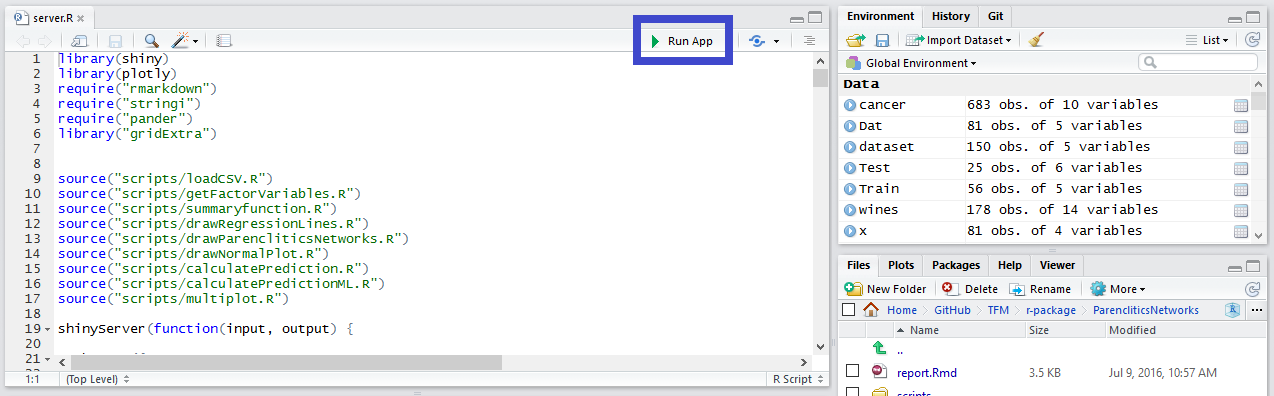
\includegraphics[width=0.7\linewidth]{imagenes/runapp}
		\caption{Hacer click en \textit{Run App}}
		\label{fig:runapp}
	\end{figure}
	
	\item Hacer click en \textit{Publish} (Figura~\ref{fig:publish}). R pedirá instalar unos paquetes necesarios para desplegar la aplicación. Respondemos afirmativamente.
	
	\begin{figure}[htbp!]
		\centering
		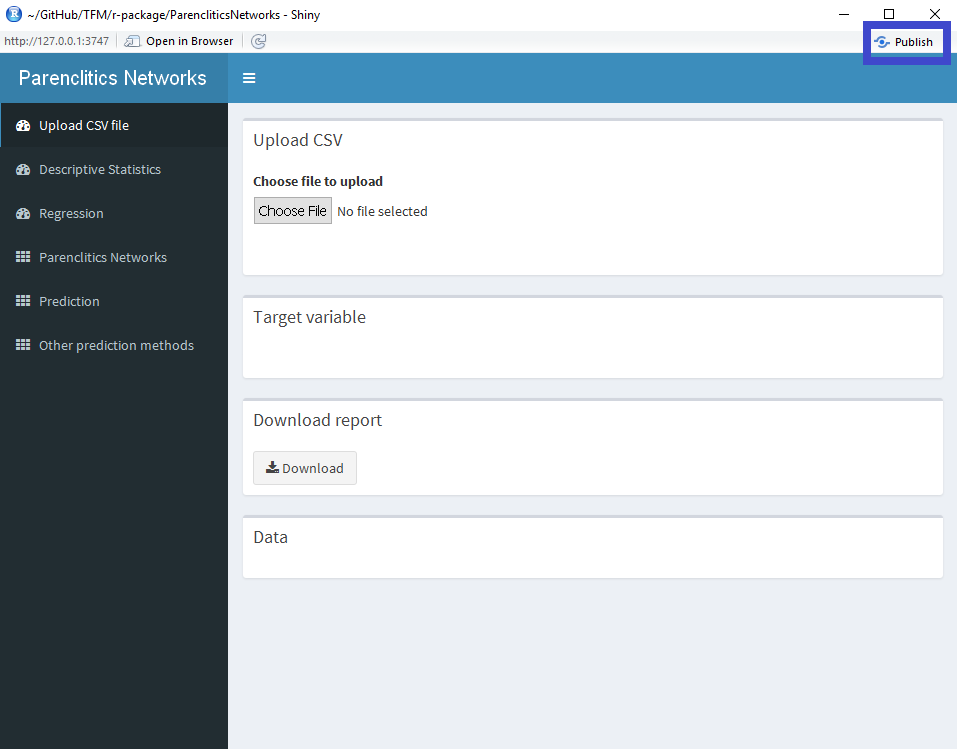
\includegraphics[width=0.7\linewidth]{imagenes/publish}
		\caption{Hacer click en \textit{Publish}}
		\label{fig:publish}
	\end{figure}
	
	\item Crear una cuenta en \url{www.shinyapps.io}.
	
	\item Dar un nombre al dominio.
	
	\item Hacer click en la opción \textit{Tokens} del menú \textit{Account}. Hacer click en \textit{Show} y en \textit{Copy to clipboard}.
	
	\item Pegar en el cuadro de texto de RStudio y hacer click en \textit{Ok}.
	
	\item Tras unos minutos, la aplicación estará desplegada en la nube.
	
\end{enumerate}